\chapter*{Annexe du chapitre \ref{chap:methodes}: Définition de la fonction de score }
\label{annexe:score}
Nous détaillons ici, le dispositif de définition de la fonction de score. 

\subsubsection{Définition de groupes}
\label{sub:group}
L'utilisateur peut définir des groupes au sein du système. Un groupe se définit en donnant la liste des positions qu'il contient dans la balise \verb!<Group_Definition>!. Par exemple:\\
\verb!<Group_Definition>! \\
\verb!grp1 1-3! \\
\verb!grp2 4 5! \\
\verb!grp3 6-8! \\
\verb!</Group_Definition>! \\
On peut définir plusieurs groupes associés à un même ensemble de positions:\\
\verb!<Group_Definition>! \\
... \\
\verb!grp3 6-8! \\
\verb!grp4 6-8! \\
\verb!</Group_Definition>! \\
Dans l'exemple précédent, grp4 représente une seconde conformation-séquence des résidus 6 à 8. Les groupes grp3, grp4 ont tous deux leur propre espace d'états, qui peuvent être différents:\\
\verb!<Space_Constraints>! \\
\verb!grp3.6  LEU TRP! \\
\verb!grp4.6  ASN ARG!  \\
\verb!</Space_Constraints>! \\
Il peut au contraire relier leurs états respectifs:\\
\verb!<Space_Constraints>! \\
\verb!grp4.TYPE grp3! \\
\verb!</Space_Constraints>! \\
La déclaration précédente garantit que grp3 et grp4 auront des séquences identiques tout au long de l'exploration.

En tirant parti de la décomposition par paires de la fonction d'énergie, on peut exprimer simplement l'énergie d'un groupe et l'interaction entre deux groupes. On a:

\begin{equation}
E(grp_i) = \sum_{a \in grp_i}E_a + \sum_{a\in grp_i} \sum_{b\in grp_i, a < b}E_{a,b} \\
\end{equation}
et
\begin{equation}
E(grp_i,grp_j) = \sum_{a \in grp_i} \sum_{b \in grp_j} E_{a,b} \\
\end{equation}
avec $E(grp_i)$ l'énergie du groupe $grp_i$, $E(grp_i,grp_j)$ l'énergie d'interaction entre les groupes $grp_i$ et $grp_j$, $E_a$ l'énergie propre du résidu $a$ et $E_{a,b}$ l'énergie d'interaction entre les rotamères aux positions $a$ et $b$. On voit les énergies de groupes sur la matrice d'énergies, figure \ref{fig:matrix_grp}. Les contributions d'un groupe se situent dans un carré sur la diagonale et les contributions à l'énergie d'interaction entre deux groupes se situent hors de la diagonale.


   \begin{figure}[!htbp]
     \centering
     \begin{tabular}{cc}
       \includegraphics[width=12cm]{figure/grp_matrix.png} &
     \end{tabular}
     
     \caption{\textbf{Les contributions aux énergies de groupes et d'interaction entre groupes dans la matrice d'énergie.} L'énergie des groupes orange, bleu et vert est une somme de termes situés des carrés de même couleur dans la matrice d'énergie. L'interaction entre le groupe bleu et le groupe vert est la somme de tous les termes du rectangle rouge.}
\label{fig:matrix_grp}
   \end{figure}
   

\subsubsection{Déclaration de la fonction de score}
\label{sub:score}
On peut introduire une nouvelle matrice qui rassemble les énergies des groupes et les énergies d'interaction entre les groupes, voir la figure \ref{fig:matrix_grp}. Dans cette matrice, l'énergie propre d'un groupe est un élément de la diagonale, celle d'une interaction entre groupes, un élément hors de la diagonale. La fonction de score peut se définir comme une combinaison linéaire des éléments de cette matrice:\\
\verb!<Optimization_Configuration>! \\
\verb!m(0.2grp1+0.2grp2+0.3grp2~grp3-0.3grp2~grp4)! \\
\verb!</Optimization_Configuration>! \\
Ici la notation de l'énergie d'interaction entre deux groupes \verb!grp2! et \verb!grp3! est \verb!grp2~grp3! et l'énergie propre du groupe \verb!grp1! est simplement \verb!grp1!. Les nombres sont des pondérations des énergies. La notation \verb!m(E)! indique que la fonction de score demandée est une minimisation de la somme déclarée entre les parenthèses. Cela signifie que pour deux séquences-conformations A et B, A est meilleure que B si $E(A) < E(B)$. Cette convention intervient dans l'exploration MSD. On peut utiliser \verb!t(...)! pour indiquer une fonction de seuil:\\
\verb!<Optimization_Configuration>! \\
\verb!t(grp1)<125.8! \\
\verb!</Optimization_Configuration>! \\
A est meilleure que B si $E(A)<125,8$. C'est utile dans le cas de l'algorithme MSD, cela permet d'obtenir un ensemble de conformations-séquences avec une énergie inférieure à un seuil.
\begin{figure}[!htbp]
  \centering
  \begin{tabular}{cc}
    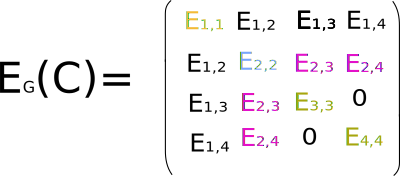
\includegraphics[width=5cm]{figure/group_matrix.png} &
  \end{tabular}
  
  \caption{\textbf{La matrice des énergies de groupe.} Les énergies des groupes grp1, grp2, grp3 et grp4 et leurs interactions présentées sous forme de matrice. Il n'y a pas d'interaction entre grp3 et grp4 parce qu'ils sont associés à un même sous-système (dupliqué).}
  \label{fig:groupmatrix}
\end{figure}



%%% Local Variables:
%%% mode: latex
%%% TeX-master: "these"
%%% End:
